\begin{figure}[htbp]
    \caption{Impact of Departures on Others}
    \label{fig:prs_opened_other_contr}
    \centering
    \begin{minipage}[b]{0.49\textwidth}
        \centering
        \subcaption{Joined pre-departure} \label{fig:predep_prs_opened_collab}
        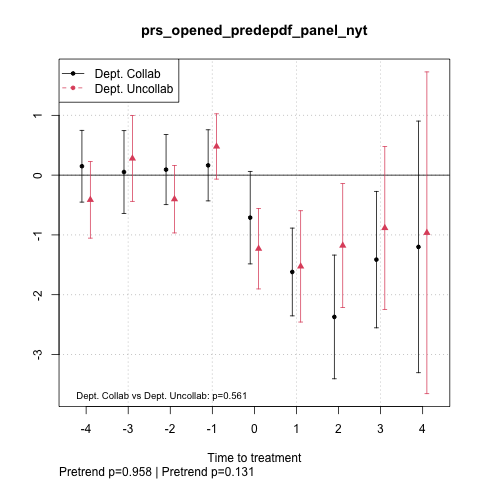
\includegraphics[width=\textwidth]{temp/output/collab/cs_norm_prs_opened_predep.png}
    \end{minipage}
    \hfill
    \begin{minipage}[b]{0.49\textwidth}
        \centering
        \subcaption{All but departed} \label{fig:nondep_prs_opened_collab}
        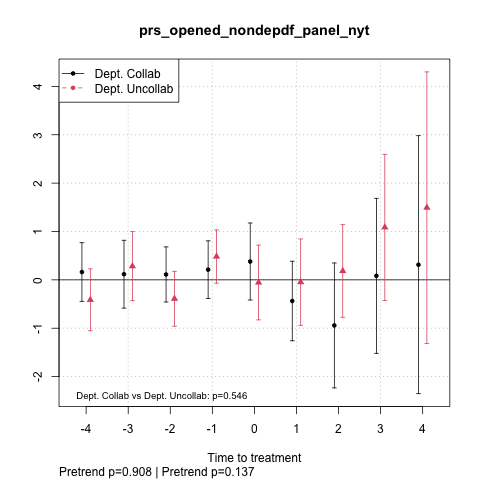
\includegraphics[width=\textwidth]{temp/output/collab/cs_norm_prs_opened_nondep.png}
    \end{minipage}

  \vspace{1ex}
  \centering
  \begin{minipage}{1\textwidth}
    \textbf{Figure notes:} 
    Following Callaway and Sant’Anna (2021), I estimate event-study coefficients accompanied by 95\% simultaneous confidence bands. For each plot with event study estimates from two subsamples, I report three Wald-test p-values: one for the pretrend test in the first subsample, one for the pretrend test in the second subsample (both from Equation \ref{eq:wald_test_pretrends} in Section \ref{sec:main_method}), and one for the difference in treatment effects across subsamples (Equation \ref{eq:wald_test} in Section \ref{sec:att_subset}). Panel~\subref{fig:predep_prs_opened_collab} depicts event study estimates from replacing the standardized outcome’s total pull request count with that of the \textbf{Pre-departure} member subset (Section~\ref{sec:contr_subset}). Panel~\subref{fig:all_prs_opened_collab} depicts event study estimates from replacing the standardized outcome’s total pull request count with that of the \textbf{Non-departure} member subset (Section~\ref{sec:contr_subset}). Both panels depict separate event study estimates for organizations with high and low departed collaborativeness. 
  \end{minipage}
\end{figure}
